\documentclass[10pt,a4paper]{article}
\usepackage[margin=17mm]{geometry}
\usepackage{graphicx}
\usepackage{booktabs}
\usepackage{microtype}
\usepackage[T1]{fontenc}
\usepackage{lmodern}
\setlength{\parindent}{0pt}
\setlength{\parskip}{5pt}
\begin{document}
\begin{center}
{\Large Isolated paired Kummer validation replay}\\[3pt]
{\small run-20261022T1354Z \quad 2026-10-22 UTC}
\end{center}

\textbf{Question.} Does the retained, byte-pinned \texttt{paired\_uncached}
executable reproduce the archived uncached candidate and same-process
negation-rho records on an isolated copy of all 1,260 public workloads?

\textbf{Run boundary.} Source commit \texttt{c63f7ed98cd9}; executable
SHA-256 \texttt{87d724fd89fa8d22...}. The command was
\texttt{timeout 3600 env -u KUMMER\_TARGET\_CAP ./paired\_uncached.original}.
The first copy-only launch exited 101 before any target because its theta-model
input was missing. After adding that pinned input, the complete run exited 0.
The host was a shared Intel Xeon 6975P-C with 32 visible logical CPUs; no
exclusive CPU reservation was earned.

\textbf{Observed output.} The second launch printed
\texttt{completed=1260 solved=1260} and \texttt{paired\_rho=1260}.
All seven candidate and seven rho JSONL files match the archived SHA-256
digests. An independent Rust analyzer reproduced all five analysis files byte
for byte, including the replay certificate, validator report, 288 price rows,
and 45,360 target-price rows. The original study validation gate passes on
materialized inputs.

\begin{center}
\begin{tabular}{ll}
\toprule
Resource telemetry, this single replay & Recorded value \\
\midrule
Wall elapsed & 24:50.16 \\
User CPU & 1471.89 s \\
System CPU & 18.32 s \\
Maximum resident memory & 287,748 KiB \\
\bottomrule
\end{tabular}
\end{center}

\textbf{Interpretation.} The price graph on page 2 is unchanged because its
raw and analyzed inputs reproduced exactly. Across 36 pooled price cells,
the modeled cold candidate/rho ratio is 8.959687--55.935424; at
$S/M=0.5$, $I/M=10$ and 0.1 GAE per native logical operation it is 14.356662.
These are operation-cost model ratios, not wall-time ratios. The run does not
prove the formulas for arbitrary curves or demonstrate a practical-size attack.
The displayed CSV has 45,360 full-cold target-price losses. Its online-only
column has 94 individual target-price wins, while all 36 pooled online cells
still lose.

\textbf{Lean proof boundary.} The pinned Lean 4.34.1 theorem
\texttt{pooled\_loss\_of\_target\_losses} proves that nonempty aligned
natural-number price lists with a strict candidate loss at every target have
a strict pooled loss. The repository axiom gate passed. The archived
floating-point CSV values and Kummer group formulas are not formal inputs to
that theorem, so it does not certify the numerical ratio band.

\textbf{Evidence.} The adjacent \texttt{RUN.md} links the input, output,
resource and failure logs; the study's \texttt{MATCHED\_REPORT.md},
\texttt{VALIDATION.json} and \texttt{plot.py} hold the original comparison,
validation gate and graph source.

\clearpage
\begin{center}
{\large Archived price graph, reproduced inputs}\par
{\small 1,260 public targets; 36 whole-cohort price cells; GAE model units}
\end{center}
\vspace{8mm}
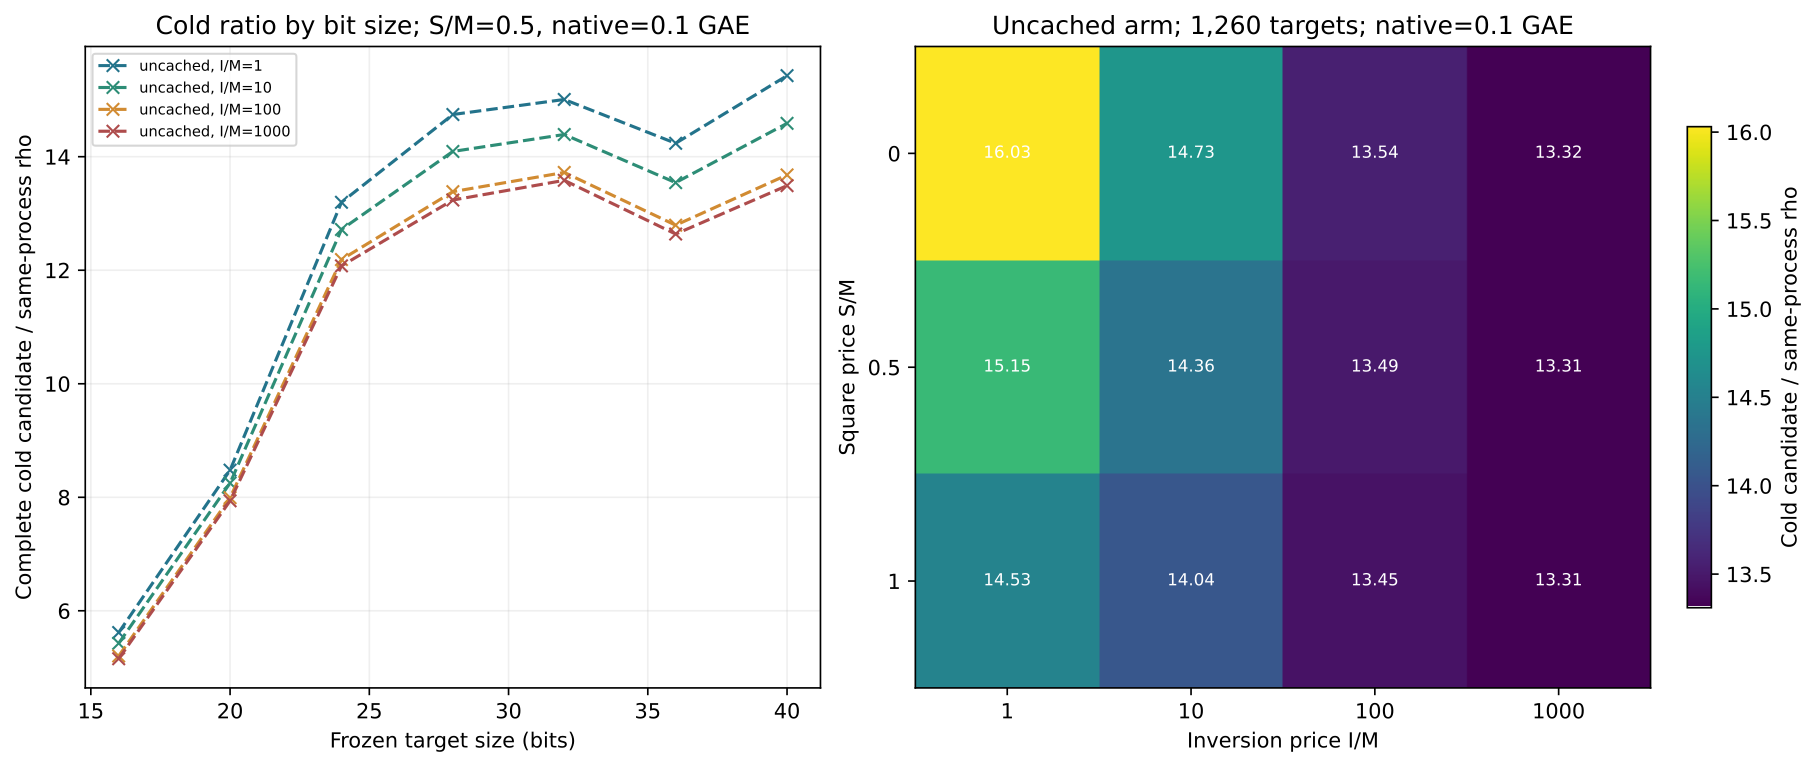
\includegraphics[width=\textwidth]{collector-cost-paired.png}
\vspace{4mm}

The candidate's full cold cost includes model, theta and torsion setup charged
per target, source transfer, signed anchor, quotient collector and verification.
The rho control is the same-process native negation solver on the same workload
IDs. The graph is reused from the study because the fresh replay's 14 raw and
five analysis files are byte-identical to the archive.
\end{document}
